\section{Special Attacks}
This section covers grappling, feinting, mounted combats, and all other forms of special attacks.

\Table{Special Attacks}{lX}{
\tableheader Special Attack & \tableheader Brief Description\\
Aid another & Grant an ally advantage on attacks or give disadvantage on an enemy's\\
Bull rush & Push an opponent back 1.5 meter or more\\
Charge & Move up to twice your speed and attack with a +2 bonus\\
Disarm & Knock a weapon from your opponent's hands, or grab a worn item\\
Feint & Negate your opponent's Dex bonus to AC\\
Grapple & Wrestle with an opponent\\
Mounted Combat & Fight while riding your steed\\
Overrun & Plow past or over an opponent as you move\\
Sunder & Strike an opponent's weapon or shield\\
Throw splash weapon & Throw container of dangerous liquid at target\\
Trip & Trip an opponent\\
Turn/rebuke undead & Channel positive (or negative) energy to turn away (or awe) undead\\
Two-weapon fighting & Fight with a weapon in each hand\\
}
\subsection{Aid Another}
In melee combat, you can help a friend attack or defend by distracting or interfering with an opponent. If you're in position to make a melee attack on an opponent that is engaging a friend in melee combat, you can attempt to aid your friend as a standard action. You make an attack roll against AC 10. If you succeed, your friend gains either gains advantage on his next attack roll against that opponent or that opponent has disadvantage on their next attack against your friend (your choice), as long as that attack comes before the beginning of your next turn. Multiple characters can aid the same friend, and similar bonuses stack.

You can also use this standard action to help a friend in other ways, such as when he is affected by a spell, or to assist another character's skill check.
\subsection{Bull Rush}
You can make a bull rush as a standard action (an attack) or as part of a charge. When you make a bull rush, you attempt to push an opponent straight back instead of damaging him. You can only bull rush an opponent who is one size category larger than you, the same size, or smaller.

\textbf{Initiating a Bull Rush:} First, you move into the defender's space. Doing this provokes an attack of opportunity from each opponent that threatens you, including the defender. (If you have the \feat{Improved Bull Rush} feat, you don't provoke an attack of opportunity from the defender.) Any attack of opportunity made by anyone other than the defender against you during a bull rush has a 25\% chance of accidentally targeting the defender instead, and any attack of opportunity by anyone other than you against the defender likewise has a 25\% chance of accidentally targeting you. (When someone makes an attack of opportunity, make the attack roll and then roll to see whether the attack went astray.)

Second, you and the defender make opposed Strength checks. You each add a +4 bonus for each size category you are larger than Medium or a $-4$ penalty for each size category you are smaller than Medium. You get advantage on your check if you are charging. The defender gets advantage on his roll if he has more than two legs or is otherwise exceptionally stable.

\textbf{Bull Rush Results:} If you beat the defender's Strength check result, you push him back 1.5 meter. If you wish to move with the defender, you can push him back an additional 1.5 meter for each 5 points by which your check result is greater than the defender's check result. You can't, however, exceed your normal movement limit. (Note: The defender provokes attacks of opportunity if he is moved. So do you, if you move with him. The two of you do not provoke attacks of opportunity from each other, however.)

If you fail to beat the defender's Strength check result, you move 1.5 meter straight back to where you were before you moved into his space. If that space is occupied, you fall prone in that space.
\subsection{Charge}
Charging is a special full-round action that allows you to move up to twice your speed and attack during the action. However, it carries tight restrictions on how you can move.

\textbf{Movement During a Charge:} You must move before your attack, not after. You must move at least 3 meters (2 squares) and may move up to double your speed directly toward the designated opponent.

You must have a clear path toward the opponent, and nothing can hinder your movement (such as difficult terrain or obstacles). Here's what it means to have a clear path. First, you must move to the closest space from which you can attack the opponent. (If this space is occupied or otherwise blocked, you can't charge.) Second, if any line from your starting space to the ending space passes through a square that blocks movement, slows movement, or contains a creature (even an ally), you can't charge. (Helpless creatures don't stop a charge.)

If you don't have line of sight to the opponent at the start of your turn, you can't charge that opponent.

You can't take a 1.5-meter step in the same round as a charge.

If you are able to take only a standard action or a move action on your turn, you can still charge, but you are only allowed to move up to your speed (instead of up to double your speed). You can't use this option unless you are restricted to taking only a standard action or move action on your turn.

\textbf{Attacking on a Charge:} After moving, you may make a single melee attack. You get a +2 bonus on the attack roll and take a $-2$ penalty to your AC until the start of your next turn.

A charging character gets advantage on the Strength check made to bull rush an opponent.

Even if you have extra attacks, such as from having a high enough base attack bonus or from using multiple weapons, you only get to make one attack during a charge.

\textbf{Lances and Charge Attacks:} A lance deals double damage if employed by a mounted character in a charge.

\textbf{Weapons Readied against a Charge:} Spears, tridents, and certain other piercing weapons deal double damage when readied (set) and used against a charging character.
\subsection{Disarm}
As a melee attack, you may attempt to disarm your opponent. If you do so with a weapon, you knock the opponent's weapon out of his hands and to the ground. If you attempt the disarm while unarmed, you end up with the weapon in your hand.

If you're attempting to disarm a melee weapon, follow the steps outlined here. If the item you are attempting to disarm isn't a melee weapon the defender may still oppose you with an attack roll, but takes a penalty and can't attempt to disarm you in return if your attempt fails.

\begin{enumerate*}
\item \textbf{Attack of Opportunity.} You provoke an attack of opportunity from the target you are trying to disarm. (If you have the \feat{Improved Disarm} feat, you don't incur an attack of opportunity for making a disarm attempt.) If the defender's attack of opportunity deals any damage, your disarm attempt fails.

\item \textbf{Opposed Rolls.} You and the defender make opposed attack rolls with your respective weapons. The wielder of a two-handed weapon on a disarm attempt gets advantage on this roll, and the wielder of a light weapon get disadvantage on the roll. (An unarmed strike is considered a light weapon, so you always get disadvantage when trying to disarm an opponent by using an unarmed strike.) If the combatants are of different sizes, the larger combatant gets a bonus on the attack roll of +4 per difference in size category. If the targeted item isn't a melee weapon, the defender gets disadvantage on the roll.

\item \textbf{Consequences.} If you beat the defender, the defender is disarmed. If you attempted the disarm action unarmed, you now have the weapon. If you were armed, the defender's weapon is on the ground in the defender's square.
\end{enumerate*}

If you fail on the disarm attempt, the defender may immediately react and attempt to disarm you with the same sort of opposed melee attack roll. His attempt does not provoke an attack of opportunity from you. If he fails his disarm attempt, you do not subsequently get a free disarm attempt against him.

\textit{Note:} A defender wearing spiked gauntlets can't be disarmed. A defender using a weapon attached to a locked gauntlet gets a +10 bonus to resist being disarmed.

\subsubsection{Grabbing Items}
You can use a disarm action to snatch an item worn by the target. If you want to have the item in your hand, the disarm must be made as an unarmed attack.

If the item is poorly secured or otherwise easy to snatch or cut away the attacker gets a +4 bonus. Unlike on a normal disarm attempt, failing the attempt doesn't allow the defender to attempt to disarm you. This otherwise functions identically to a disarm attempt, as noted above.

You can't snatch an item that is well secured unless you have pinned the wearer (see Grapple). Even then, the defender gains a +4 bonus on his roll to resist the attempt.
\subsection{Feint}
Feinting is a standard action. To feint, make a \skill{Bluff} check opposed by a \skill{Sense Motive} check by your target. The target may add his base attack bonus to this \skill{Sense Motive} check. If your \skill{Bluff} check result exceeds your target's \skill{Sense Motive} check result, the next melee attack you make against the target does not allow him to use his Dexterity bonus to AC (if any). This attack must be made on or before your next turn.

When feinting in this way against a creature of a different shape than yours, you get disadvantage on your roll. For example, an elf would get disadvantage on her \skill{Bluff} check to feint a thri-kreen, since she is humanoid and he is a insectoid. At the same time, he would roll with disadvantage if he tries to feint the elf.

Against a creature of animal Intelligence (1 or 2), you take a $-8$ penalty. Against a nonintelligent creature, it's impossible.

Feinting in combat does not provoke attacks of opportunity.

\textbf{Feinting as a Move Action:} With the \feat{Improved Feint} feat, you can attempt a feint as a move action instead of as a standard action.
\subsection{Grapple}
Grappling is holding an opponent in hand-to-hand combat, very common in smaller gladiatorial arenas. For monsters, it can mean locking you in its mouth, or holding you down in the ground.

\subsubsection{Grapple Checks}
Repeatedly in a grapple, you need to make opposed grapple checks against an opponent. A grapple check is like a melee attack roll. Your attack bonus on a grapple check is:

{
	\centering
	\vskip1em
	\Large \textit{Base attack bonus} + \textit{Str. modifier}\\ + \textit{special size modifier}
	\vskip1em
}

\textbf{Special Size Modifier:} The special size modifier for a grapple check is as follows: Colossal +16, Gargantuan +12, Huge +8, Large +4, Medium +0, Small $-4$, Tiny $-8$, Diminutive $-12$, Fine $-16$. Use this number in place of the normal size modifier you use when making an attack roll.

\subsubsection{Starting a Grapple}
To start a grapple, you need to grab and hold your target. Starting a grapple requires a successful melee attack roll. If you get multiple attacks, you can attempt to start a grapple multiple times (at successively lower base attack bonuses).

\begin{enumerate*}
\item \textbf{Attack of Opportunity.} You provoke an attack of opportunity from the target you are trying to grapple. If the attack of opportunity deals damage, the grapple attempt fails. (Certain monsters do not provoke attacks of opportunity when they attempt to grapple, nor do characters with the Improved Grapple feat.) If the attack of opportunity misses or fails to deal damage, proceed to Step 2.

\item \textbf{Grab.} You make a melee touch attack to grab the target. If you fail to hit the target, the grapple attempt fails. If you succeed, proceed to Step 3.

\item \textbf{Hold.} Make an opposed grapple check as a free action. If you succeed, you and your target are now grappling, and you deal damage to the target as if with an unarmed strike.

If you lose, you fail to start the grapple. You automatically lose an attempt to hold if the target is two or more size categories larger than you are.

In case of a tie, the combatant with the higher grapple check modifier wins. If this is a tie, roll again to break the tie.

\item \textbf{Maintain Grapple.} To maintain the grapple for later rounds, you must move into the target's space. (This movement is free and doesn't count as part of your movement in the round.) Moving, as normal, provokes attacks of opportunity from threatening opponents, but not from your target.

If you can't move into your target's space, you can't maintain the grapple and must immediately let go of the target. To grapple again, you must begin at Step 1.
\end{enumerate*}

\subsubsection{Grappling Consequences}
While you're grappling, your ability to attack others and defend yourself is limited.

\textbf{No Threatened Squares:} You don't threaten any squares while grappling.

\textbf{No Dexterity Bonus:} You lose your Dexterity bonus to AC (if you have one) against opponents you aren't grappling. (You can still use it against opponents you are grappling.)

\textbf{No Movement:} You can't move normally while grappling. You may, however, make an opposed grapple check to move while grappling.

\subsubsection{If You're Grappling}
When you are grappling (regardless of who started the grapple), you can perform any of the following actions. Some of these actions take the place of an attack (rather than being a standard action or a move action). If your base attack bonus allows you multiple attacks, you can attempt one of these actions in place of each of your attacks, but at successively lower base attack bonuses.

\textbf{Activate a Magic Item:} You can activate a magic item, as long as the item doesn't require spell completion activation. You don't need to make a grapple check to activate the item.

\textbf{Attack Your Opponent:} You can make an attack with an unarmed strike, natural weapon, or light weapon against another character you are grappling. You take a $-4$ penalty on such attacks.

You can't attack with two weapons while grappling, even if both are light weapons.

\textbf{Cast a Spell:} You can attempt to cast a spell while grappling or even while pinned (see below), provided its casting time is no more than 1 standard action, it has no somatic component, and you have in hand any material components or focuses you might need. Any spell that requires precise and careful action is impossible to cast while grappling or being pinned. If the spell is one that you can cast while grappling, you must make a Concentration check (DC 20 + spell level) or lose the spell. You don't have to make a successful grapple check to cast the spell.

\textbf{Damage Your Opponent:} While grappling, you can deal damage to your opponent equivalent to an unarmed strike. Make an opposed grapple check in place of an attack. If you win, you deal nonlethal damage as normal for your unarmed strike (1d3 points for Medium attackers or 1d2 points for Small attackers, plus Strength modifiers). If you want to deal lethal damage, you take a $-4$ penalty on your grapple check.

\textit{Exception:} Monks deal more damage on an unarmed strike than other characters, and the damage is lethal. However, they can choose to deal their damage as nonlethal damage when grappling without taking the usual $-4$ penalty for changing lethal damage to nonlethal damage.

\textbf{Draw a Light Weapon:} You can draw a light weapon as a move action with a successful grapple check.

\textbf{Escape from Grapple:} You can escape a grapple by winning an opposed grapple check in place of making an attack. You can make an Escape Artist check in place of your grapple check if you so desire, but this requires a standard action. If more than one opponent is grappling you, your grapple check result has to beat all their individual check results to escape. (Opponents don't have to try to hold you if they don't want to.) If you escape, you finish the action by moving into any space adjacent to your opponent(s).

\textbf{Move:} You can move half your speed (bringing all others engaged in the grapple with you) by winning an opposed grapple check. This requires a standard action, and you must beat all the other individual check results to move the grapple.

\textit{Note:} You get a +4 bonus on your grapple check to move a pinned opponent, but only if no one else is involved in the grapple.

\textbf{Retrieve a Spell Component:} You can produce a spell component from your pouch while grappling by using a full-round action. Doing so does not require a successful grapple check.

\textbf{Pin Your Opponent:} You can hold your opponent immobile for 1 round by winning an opposed grapple check (made in place of an attack). Once you have an opponent pinned, you have a few options available to you (see below).

\textbf{Break Another's Pin:} If you are grappling an opponent who has another character pinned, you can make an opposed grapple check in place of an attack. If you win, you break the hold that the opponent has over the other character. The character is still grappling, but is no longer pinned.

\textbf{Use Opponent's Weapon:} If your opponent is holding a light weapon, you can use it to attack him. Make an opposed grapple check (in place of an attack). If you win, make an attack roll with the weapon with a $-4$ penalty (doing this doesn't require another action).

You don't gain possession of the weapon by performing this action.

\subsubsection{If You're Pinning an Opponent}
You can attempt to damage your opponent with an opposed grapple check, you can attempt to use your opponent's weapon against him, or you can attempt to move the grapple (all described above). At your option, you can prevent a pinned opponent from speaking.

You can use a disarm action to remove or grab away a well secured object worn by a pinned opponent, but he gets a +4 bonus on his roll to resist your attempt.

You may voluntarily release a pinned character as a free action; if you do so, you are no longer considered to be grappling that character (and vice versa).

You can't draw or use a weapon (against the pinned character or any other character), escape another's grapple, retrieve a spell component, pin another character, or break another's pin while you are pinning an opponent.

\Figure*{b}{images/raiders-1.png}

\subsubsection{If You're Pinned by an Opponent}
When an opponent has pinned you, you are held immobile (but not helpless) for 1 round. While you're pinned, you take a $-4$ penalty to your AC against opponents other than the one pinning you. At your opponent's option, you may also be unable to speak. On your turn, you can try to escape the pin by making an opposed grapple check in place of an attack. You can make an Escape Artist check in place of your grapple check if you want, but this requires a standard action. If you win, you escape the pin, but you're still grappling.

\subsubsection{Joining a Grapple}
If your target is already grappling someone else, you can use an attack to start a grapple, as above, except that the target doesn't get an attack of opportunity against you, and your grab automatically succeeds. You still have to make a successful opposed grapple check to become part of the grapple.

If there are multiple opponents involved in the grapple, you pick one to make the opposed grapple check against.

\subsubsection{Multiple Grapplers}
Several combatants can be in a single grapple. Up to four combatants can grapple a single opponent in a given round. Creatures that are one or more size categories smaller than you count for half, creatures that are one size category larger than you count double, and creatures two or more size categories larger count quadruple.

When you are grappling with multiple opponents, you choose one opponent to make an opposed check against. The exception is an attempt to escape from the grapple; to successfully escape, your grapple check must beat the check results of each opponent.
\begin{figure*}[t!]
\centering
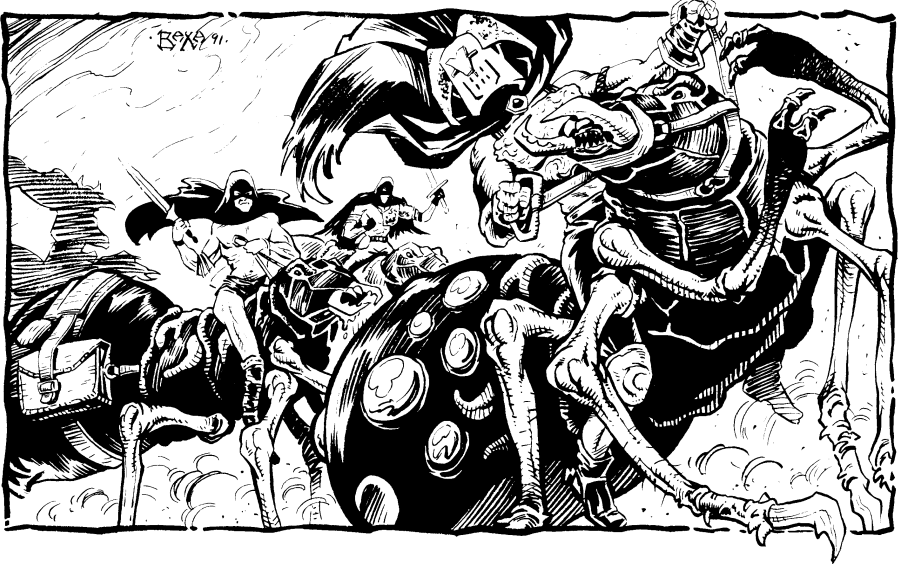
\includegraphics[width=\textwidth]{images/raiders-1.png}
\WOTC
\end{figure*}
% \Figure*{t}{images/raiders-1.png}
\subsection{Mounted Combat}
\textbf{Horses in Combat:} Heavy warhorses, light warhorses and warponies can serve readily as combat steeds. Light horses, ponies, and heavy horses, however, are frightened by combat. If you don't dismount, you must make a DC 20 \skill{Ride} check each round as a move action to control such a horse. If you succeed, you can perform a standard action after the move action. If you fail, the move action becomes a full round action and you can't do anything else until your next turn.

Your mount acts on your initiative count as you direct it. You move at its speed, but the mount uses its action to move.

A horse (not a pony) is a Large creature and thus takes up a space 3 meters (2 squares) across. For simplicity, assume that you share your mount's space during combat.

\textbf{Combat while Mounted:} With a DC 5 \skill{Ride} check, you can guide your mount with your knees so as to use both hands to attack or defend yourself. This is a free action.

When you attack a creature smaller than your mount that is on foot, you get the +1 bonus on melee attacks for being on higher ground. If your mount moves more than 1.5 meter, you can only make a single melee attack. Essentially, you have to wait until the mount gets to your enemy before attacking, so you can't make a full attack. Even at your mount's full speed, you don't take any penalty on melee attacks while mounted.

If your mount charges, you also take the AC penalty associated with a charge. If you make an attack at the end of the charge, you receive the bonus gained from the charge. When charging on horseback, you deal double damage with a lance.

You can use ranged weapons while your mount is taking a double move, but at a $-4$ penalty on the attack roll. You can use ranged weapons while your mount is running (quadruple speed), at a $-8$ penalty. In either case, you make the attack roll when your mount has completed half its movement. You can make a full attack with a ranged weapon while your mount is moving. Likewise, you can take move actions normally.

\textbf{Casting Spells while Mounted:} You can cast a spell normally if your mount moves up to a normal move (its speed) either before or after you cast. If you have your mount move both before and after you cast a spell, then you're casting the spell while the mount is moving, and you have to make a \skill{Concentration} check due to the vigorous motion (DC 10 + spell level) or lose the spell. If the mount is running (quadruple speed), you can cast a spell when your mount has moved up to twice its speed, but your \skill{Concentration} check is more difficult due to the violent motion (DC 15 + spell level).

\textbf{If Your Mount Falls in Battle:} If your mount falls, you have to succeed on a DC 15 \skill{Ride} check to make a soft fall and take no damage. If the check fails, you take 1d6 points of damage.

\textbf{If You Are Dropped:} If you are knocked unconscious, you have a 50\% chance to stay in the saddle (or 75\% if you're in a military saddle). Otherwise you fall and take 1d6 points of damage.

Without you to guide it, your mount avoids combat.
\subsection{Overrun}
You can attempt an overrun as a standard action taken during your move. (In general, you cannot take a standard action during a move; this is an exception.) With an overrun, you attempt to plow past or over your opponent (and move through his square) as you move. You can only overrun an opponent who is one size category larger than you, the same size, or smaller. You can make only one overrun attempt per round.

If you're attempting to overrun an opponent, follow these steps.

\begin{enumerate*}
\item \textbf{Attack of Opportunity.} Since you begin the overrun by moving into the defender's space, you provoke an attack of opportunity from the defender.

\item \textbf{Opponent Avoids?} The defender has the option to simply avoid you. If he avoids you, he doesn't suffer any ill effect and you may keep moving (You can always move through a square occupied by someone who lets you by.) The overrun attempt doesn't count against your actions this round (except for any movement required to enter the opponent's square). If your opponent doesn't avoid you, move to Step 3.

\item \textbf{Opponent Blocks?} If your opponent blocks you, make a Strength check opposed by the defender's Dexterity or Strength check (whichever ability score has the higher modifier). A combatant gets a +4 bonus on the check for every size category he is larger than Medium or a $-4$ penalty for every size category he is smaller than Medium. The defender gets advantage on his check if he has more than two legs or is otherwise more stable than a normal humanoid. If you win, you knock the defender prone. If you lose, the defender may immediately react and make a Strength check opposed by your Dexterity or Strength check (including the size modifiers noted above, but no other modifiers) to try to knock you prone.

\item \textbf{Consequences.} If you succeed in knocking your opponent prone, you can continue your movement as normal. If you fail and are knocked prone in turn, you have to move 1.5 meter back the way you came and fall prone, ending your movement there. If you fail but are not knocked prone, you have to move 1.5 meter back the way you came, ending your movement there. If that square is occupied, you fall prone in that square.
\end{enumerate*}

\textbf{Improved Overrun:} If you have the \feat{Improved Overrun} feat, your target may not choose to avoid you.

\textbf{Mounted Overrun (Trample):} If you attempt an overrun while mounted, your mount makes the Strength check to determine the success or failure of the overrun attack (and applies its size modifier, rather than yours). If you have the \feat{Trample} feat and attempt an overrun while mounted, your target may not choose to avoid you, and if you knock your opponent prone with the overrun, your mount may make one hoof attack against your opponent.
\subsection{Sunder}
You can use a melee attack with a slashing or bludgeoning weapon to strike a weapon or shield that your opponent is holding. If you're attempting to sunder a weapon or shield, follow the steps outlined here. (Attacking held objects other than weapons or shields is covered below.)

\Table{Common Armor, Weapon, and Shield Hardness and Hit Points}{X cc}{
\tableheader Weapon or Shield & \tableheader Hardness & \tableheader HP\footnotemark[1]\\
\TableSubheader{Light blade} &&\\
~ wood & 5 & 1\\
~ bone & 6 & 1\\
~ stone & 8 & 1\\
~ metal & 10 & 2\\
\TableSubheader{One-handed blade} &&\\
~ wood & 5 & 2\\
~ bone & 6 & 2\\
~ stone & 8 & 3\\
~ metal & 10 & 5\\
\TableSubheader{Two-handed blade} &&\\
~ wood & 5 & 4\\
~ bone & 6 & 4\\
~ stone & 8 & 5\\
~ metal & 10 & 10\\
\TableSubheader{Light weapon} &&\\
~ wood-hafted & 5 & 2\\
~ bone-hafted & 6 & 2\\
~ stone-hafted & 8 & 3\\
~ metal-hafted & 10 & 10\\
\TableSubheader{One-handed weapon} &&\\
~ wood-hafted & 5 & 5\\
~ bone-hafted & 6 & 5\\
~ stone-hafted & 8 & 8\\
~ metal-hafted & 10 & 20\\
\TableSubheader{Two-handed weapon} &&\\
~ wood-hafted & 5 & 10\\
~ bone-hafted & 6 & 10\\
~ stone-hafted & 8 & 15\\
Projectile weapon & 5 & 5\\
Armor & $\star$ & armor bonus $\times5$\\
Buckler & 10 & 5\\
\TableSubheader{Light shield} &&\\
~ wooden & 5 & 7\\
~ steel & 10 & 10\\
\TableSubheader{Heavy shield} &&\\
~ wooden & 5 & 15\\
~ steel & 10 & 20\\
Tower shield & 5 & 20\\

\TableNote{3}{1 The hp value given is for Medium armor, weapons, and shields. Divide by 2 for each size category of the item smaller than Medium, or multiply it by 2 for each size category larger than Medium.}\\
\TableNote{3}{$\star$ Varies by material; see \tabref{Substance Hardness and Hit Points}.}\\
}

\begin{enumerate*}
\item \textbf{Attack of Opportunity.} You provoke an attack of opportunity from the target whose weapon or shield you are trying to sunder. (If you have the \feat{Improved Sunder} feat, you don't incur an attack of opportunity for making the attempt.)

\item \textbf{Opposed Rolls.} You and the defender make opposed attack rolls with your respective weapons. The wielder of a two-handed weapon on a sunder attempt gets advantage on this roll, and the wielder of a light weapon gets disadvantage on the roll. If the combatants are of different sizes, the larger combatant gets a bonus on the attack roll of +4 per difference in size category.

\item \textbf{Consequences.} If you beat the defender, roll damage and deal it to the weapon or shield. See \tabref{Common Armor, Weapon, and Shield Hardness and Hit Points} to determine how much damage you must deal to destroy the weapon or shield.
\end{enumerate*}

If you fail the sunder attempt, you don't deal any damage.

\textbf{Sundering a Carried or Worn Object:} You don't use an opposed attack roll to damage a carried or worn object. Instead, just make an attack roll against the object's AC. A carried or worn object's AC is equal to 10 + its size modifier + the Dexterity modifier of the carrying or wearing character. Attacking a carried or worn object provokes an attack of opportunity just as attacking a held object does. To attempt to snatch away an item worn by a defender rather than damage it, see Disarm. You can't sunder armor worn by another character.
\subsection{Throw Splash Weapon}
A splash weapon is a ranged weapon that breaks on impact, splashing or scattering its contents over its target and nearby creatures or objects. To attack with a splash weapon, make a ranged touch attack against the target. Splash weapons require no weapon proficiency, so you don't take the nonproficiency disadvantage. A hit deals direct hit damage to the target, and splash damage to all creatures within 1.5 of the target.

You can instead target a specific grid intersection. Treat this as a ranged attack against AC 5. However, if you target a grid intersection, creatures in all adjacent squares are dealt the splash damage, and the direct hit damage is not dealt to any creature. (You can't target a grid intersection occupied by a creature, such as a Large or larger creature; in this case, you're aiming at the creature.)

If you miss the target (whether aiming at a creature or a grid intersection), roll 1d8. This determines the misdirection of the throw, with 1 being straight back at you and 2 through 8 counting clockwise around the grid intersection or target creature. Then, count a number of squares in the indicated direction equal to the range increment of the throw.

After you determine where the weapon landed, it deals splash damage to all creatures in adjacent squares.
\subsection{Trip}
You can try to trip an opponent as an unarmed melee attack. You can only trip an opponent who is one size category larger than you, the same size, or smaller.

\textbf{Making a Trip Attack:} Make an unarmed melee touch attack against your target. This provokes an attack of opportunity from your target as normal for unarmed attacks.

If your attack succeeds, make a Strength check opposed by the defender's Dexterity or Strength check (whichever ability score has the higher modifier). A combatant gets a +4 bonus for every size category he is larger than Medium or a $-4$ penalty for every size category he is smaller than Medium. The defender gets advantage on his check if he has more than two legs or is otherwise more stable than a normal humanoid. If you win, you trip the defender. If you lose, the defender may immediately react and make a Strength check opposed by your Dexterity or Strength check to try to trip you.

\textit{Avoiding Attacks of Opportunity:} If you have the \feat{Improved Trip} feat, or if you are tripping with a weapon (see below), you don't provoke an attack of opportunity for making a trip attack.

\textbf{Being Tripped (Prone):} A tripped character is prone. Standing up is a move action.

\textbf{Tripping a Mounted Opponent:} You may make a trip attack against a mounted opponent. The defender may make a Ride check in place of his Dexterity or Strength check. If you succeed, you pull the rider from his mount.

\textbf{Tripping with a Weapon:} Some weapons can be used to make trip attacks. In this case, you make a melee touch attack with the weapon instead of an unarmed melee touch attack, and you don't provoke an attack of opportunity.

If you are tripped during your own trip attempt, you can drop the weapon to avoid being tripped.
\subsection{Turn Or Rebuke Undead}
Good clerics and some neutral clerics can channel positive energy, which can halt, drive off (rout), or destroy undead.

Evil clerics and some neutral clerics can channel negative energy, which can halt, awe (rebuke), control (command), or bolster undead.

Regardless of the effect, the general term for the activity is ``turning.'' When attempting to exercise their divine control over these creatures, characters make turning checks.

\Table{Turning Undead}{CC}{
\tableheader Turning Check Result & \tableheader Most Powerful Undead Affected (Maximum Hit Dice)\\
0 or lower & Cleric's level $-4$ \\
1--3 & Cleric's level $-3$ \\
4--6 & Cleric's level $-2$ \\
7--9 & Cleric's level $-1$ \\
10--12 & Cleric's level \\
13--15 & Cleric's level +1 \\
16--18 & Cleric's level +2 \\
19--21 & Cleric's level +3 \\
22 or higher & Cleric's level +4 \\
}

\subsubsection{Turning Checks}
Turning undead is a supernatural ability that a character can perform as a standard action. It does not provoke attacks of opportunity.

You must present your holy symbol to turn undead. Turning is considered an attack.

\textbf{Times per Day:} You may attempt to turn undead a number of times per day equal to 3 + your Charisma modifier. You can increase this number by taking the Extra Turning feat.

\textbf{Range:} You turn the closest turnable undead first, and you can't turn undead that are more than 60 feet away or that have total cover relative to you. You don't need line of sight to a target, but you do need line of effect.

\textbf{Turning Check:} The first thing you do is roll a turning check to see how powerful an undead creature you can turn. This is a Charisma check (1d20 + your Charisma modifier). \tabref{Turning Undead} gives you the Hit Dice of the most powerful undead you can affect, relative to your level. On a given turning attempt, you can turn no undead creature whose Hit Dice exceed the result on this table.

\textbf{Turning Damage:} If your roll on \tabref{Turning Undead} is high enough to let you turn at least some of the undead within 60 feet, roll 2d6 + your cleric level + your Charisma modifier for turning damage. That's how many total Hit Dice of undead you can turn.

If your Charisma score is average or low, it's possible to roll fewer Hit Dice of undead turned than indicated on \tabref{Turning Undead}.

You may skip over already turned undead that are still within range, so that you do not waste your turning capacity on them.

\textbf{Effect and Duration of Turning:} Turned undead flee from you by the best and fastest means available to them. They flee for 10 rounds (1 minute). If they cannot flee, they cower (giving any attack rolls against them a +2 bonus). If you approach within 10 feet of them, however, they overcome being turned and act normally. (You can stand within 10 feet without breaking the turning effect---you just can't approach them.) You can attack them with ranged attacks (from at least 10 feet away), and others can attack them in any fashion, without breaking the turning effect.

\textbf{Destroying Undead:} If you have twice as many levels (or more) as the undead have Hit Dice, you destroy any that you would normally turn.

\subsubsection{Evil Clerics and Undead}
Evil clerics channel negative energy to rebuke (awe) or command (control) undead rather than channeling positive energy to turn or destroy them. An evil cleric makes the equivalent of a turning check. Undead that would be turned are rebuked instead, and those that would be destroyed are commanded.

\textbf{Rebuked:} A rebuked undead creature cowers as if in awe (attack rolls against the creature get a +2 bonus). The effect lasts 10 rounds.

\textbf{Commanded:} A commanded undead creature is under the mental control of the evil cleric. The cleric must take a standard action to give mental orders to a commanded undead. At any one time, the cleric may command any number of undead whose total Hit Dice do not exceed his level. He may voluntarily relinquish command on any commanded undead creature or creatures in order to command new ones.

\textbf{Dispelling Turning:} An evil cleric may channel negative energy to dispel a good cleric's turning effect. The evil cleric makes a turning check as if attempting to rebuke the undead. If the turning check result is equal to or greater than the turning check result that the good cleric scored when turning the undead, then the undead are no longer turned. The evil cleric rolls turning damage of 2d6 + cleric level + Charisma modifier to see how many Hit Dice worth of undead he can affect in this way (as if he were rebuking them).

\textbf{Bolstering Undead:} An evil cleric may also bolster undead creatures against turning in advance. He makes a turning check as if attempting to rebuke the undead, but the Hit Dice result on \tabref{Turning Undead} becomes the undead creatures' effective Hit Dice as far as turning is concerned (provided the result is higher than the creatures' actual Hit Dice). The bolstering lasts 10 rounds. An evil undead cleric can bolster himself in this manner.

\subsubsection{Neutral Clerics and Undead}
A cleric of neutral alignment can either turn undead but not rebuke them, or rebuke undead but not turn them. See Turn or Rebuke Undead for more information.

Even if a cleric is neutral, channeling positive energy is a good act and channeling negative energy is evil.

%Paladins and Undead
%Beginning at 4th level, paladins can turn undead as if they were clerics of three levels lower than they actually are.

\subsubsection{Turning Other Creatures}
Some clerics have the ability to turn creatures other than undead.

The turning check result is determined as normal.
\subsection{Two-Weapon Fighting}
If you wield a second weapon in your off hand, you can get one extra attack per round with that weapon. You suffer a $-6$ penalty with your regular attack or attacks with your primary hand and a $-10$ penalty to the attack with your off hand when you fight this way. You can reduce these penalties in two ways:

\begin{itemize*}
\item If your off-hand weapon is light, the penalties are reduced by 2 each. (An unarmed strike is always considered light.)
\item The \feat{Two-Weapon Fighting} feat lessens the primary hand penalty by 2, and the off-hand penalty by 6.
\end{itemize*}

\tabref{Two-Weapon Fighting Penalties} summarizes the interaction of all these factors.

\Table{Two-Weapon Fighting Penalties}{p{38mm}CC}{
\tableheader Circumstances & \tableheader Primary Hand & \tableheader Off Hand \\
Normal penalties & $-6$ & $-10$ \\
Off-hand weapon is light & $-4$ & $-8$ \\
\feat{Two-Weapon Fighting} feat & $-4$ & $-4$ \\
Off-hand weapon is light and \feat{Two-Weapon Fighting} feat & $-2$ & $-2$ \\
}

\textbf{Double Weapons:} You can use a double weapon to make an extra attack with the off-hand end of the weapon as if you were fighting with two weapons. The penalties apply as if the off-hand end of the weapon were a light weapon.

\textbf{Thrown Weapons:} The same rules apply when you throw a weapon from each hand. Treat a dart or shuriken as a light weapon when used in this manner, and treat a bolas, javelin, net, or sling as a one-handed weapon.

\textbf{Shield Bash Attacks:} You can bash an opponent with a light shield or heavy shield, using it as an off-hand weapon. See \tabref{Martial Weapons} for the damage dealt by a shield bash. Used this way, a shield is a martial bludgeoning weapon. For the purpose of penalties on attack rolls, treat a heavy shield as a one-handed weapon and a light shield as a light weapon. If you use your shield as a weapon, you lose its AC bonus until your next action (usually until the next round). An enhancement bonus on a shield does not improve the effectiveness of a shield bash made with it, but the shield can be made into a magic weapon in its own right.

\textbf{Shield Spikes:} When added to your shield, these spikes turn it into a martial piercing weapon that increases the damage dealt by a shield bash as if the shield were designed for a creature one size category larger than you. You can’t put spikes on a buckler or a tower shield. Otherwise, attacking with a spiked shield is like making a shield bash attack.

An enhancement bonus on a spiked shield does not improve the effectiveness of a shield bash made with it, but a spiked shield can be made into a magic weapon in its own right.